% ------------------------------------------------------------------------------
% TYPO3 CMS 8.1 - What's New (French Version)
%
% @author	Patrick Lobacher <patrick@lobacher.de> and Michael Schams <schams.net>
% @license	Creative Commons BY-NC-SA 3.0
% @link		http://typo3.org/download/release-notes/whats-new/
% @language	French
% ------------------------------------------------------------------------------
% LTXE-CHAPTER-UID:		dcfe6009-2200ad81-816c2edb-1f54c687
% LTXE-CHAPTER-NAME:	Backend User Interface
% ------------------------------------------------------------------------------

\section{Interface Utilisateur Backend}
\begin{frame}[fragile]
	\frametitle{Interface Utilisateur Backend}

	\begin{center}\huge{Chapitre 1~:}\end{center}
	\begin{center}\huge{\color{typo3darkgrey}\textbf{Interface Utilisateur Backend}}\end{center}

\end{frame}

% ------------------------------------------------------------------------------
% LTXE-SLIDE-START
% LTXE-SLIDE-UID:		9029b6f2-0822faed-85e4b52b-53d2a724
% LTXE-SLIDE-ORIGIN:	5d3d70fa-92a2935e-f1cbdc1e-285ec842 English
% LTXE-SLIDE-TITLE:		Feature: #75497 - inline backend layout wizard
% LTXE-SLIDE-REFERENCE:	!Feature-75497-InlineBackendLayoutWizard.rst
% ------------------------------------------------------------------------------
\begin{frame}[fragile]
	\frametitle{Interface Utilisateur Backend}
	\framesubtitle{Assistant sur place de disposition backend}

	Un nouveau type de rendu dans FormEngine est ajouté pour fournir l'assistant
	de disposition backend sur place (TCA~: \texttt{'renderType' => 'belayoutwizard'}).

	\begin{figure}
		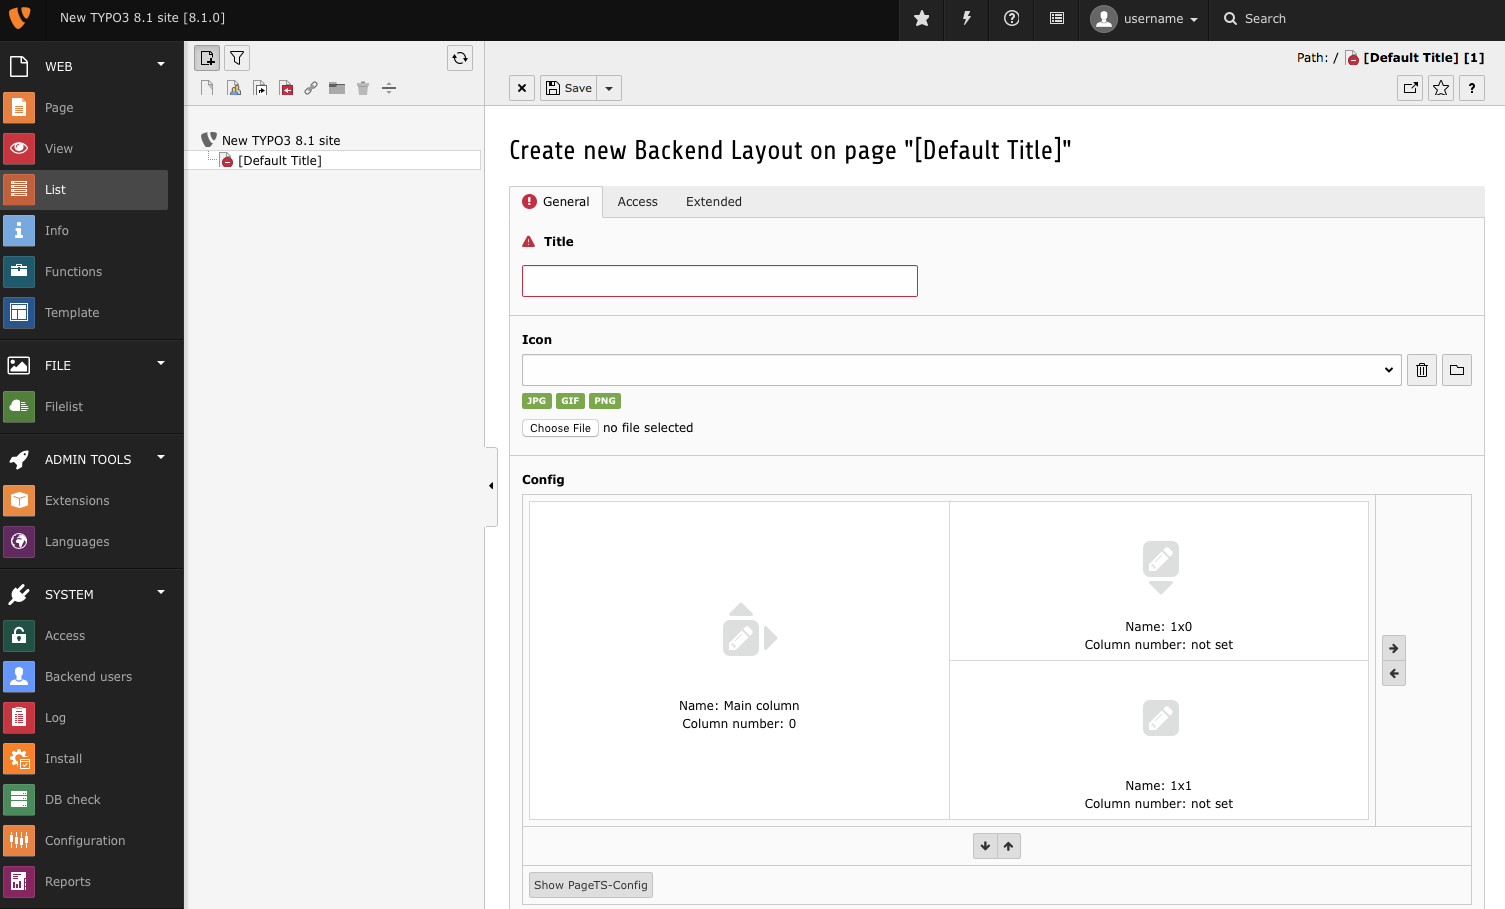
\includegraphics[width=0.70\linewidth]{BackendUserInterface/75497.png}
	\end{figure}

\end{frame}


% ------------------------------------------------------------------------------
% LTXE-SLIDE-START
% LTXE-SLIDE-UID:		c187de6d-c0d85b6b-f399d38f-1b3f9b36
% LTXE-SLIDE-ORIGIN:	7cab4dc0-cdfe9472-a3f0a874-dddf137d English
% LTXE-SLIDE-TITLE:		Feature: #75581 - Simplify cache clearing
% LTXE-SLIDE-REFERENCE:	!Feature-75581-SimplifyCacheClearing.rst
% ------------------------------------------------------------------------------
\begin{frame}[fragile]
	\frametitle{Interface Utilisateur Backend}
	\framesubtitle{Simplification du vidage de cache}

	Le système de vidage de cache est simplifié en retirant des options dans le menu de vidage
	du cache et l'outils d'installation.

	\begin{itemize}

		\item \textbf{Vider les caches Frontend~:}\newline
			\small
				Vide les caches frontend et liés aux pages, comme précédemment.
			\normalsize

		\item \textbf{Vider tous les caches~:}\newline
			\small
				Vide tous les caches système, incluant le chargeur de classe, les traductions,
				le cache des configurations d'extension et le cache d'opcode. Reconstruire ces
				caches peut prendre un certain temps.
			\normalsize

	\end{itemize}

	\begin{figure}
		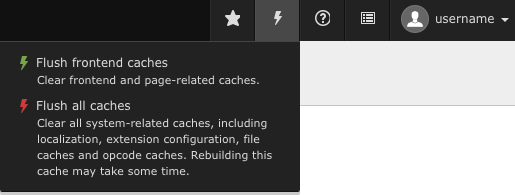
\includegraphics[width=0.45\linewidth]{BackendUserInterface/75581.png}
	\end{figure}

\end{frame}

% ------------------------------------------------------------------------------
% LTXE-SLIDE-START
% LTXE-SLIDE-UID:		5496d331-7edf6417-45d71049-dd028eb0
% LTXE-SLIDE-ORIGIN:	e24e593c-fe9bcff9-c386db3a-79491de1 English
% LTXE-SLIDE-TITLE:		Rework Workspaces (1)
% LTXE-SLIDE-REFERENCE:	Rework Workspaces
% ------------------------------------------------------------------------------
\begin{frame}[fragile]
	\frametitle{Interface Utilisateur Backend}
	\framesubtitle{Travaux sur les espaces de travail (1)}

	\begin{itemize}

		\item Le module des espaces de travail pour gérer les étapes des contenus est réécris
			et s'intègre mieux dans l'apparence visuel du backend

		\item Les éditeurs réaliseront tout de suite qu'il s'accorde avec l'apparence globale
			en raison de sa base technique sur Twitter Bootstrap et jQuery

		\item Ce changement apporte aussi un gain de performance et est un grand pas en avant
			vers un backend TYPO3 plus propre et rapide avec moins de JavaScript

	\end{itemize}

\end{frame}

% ------------------------------------------------------------------------------
% LTXE-SLIDE-START
% LTXE-SLIDE-UID:		ceab9881-24a3ca23-9784ec96-55e0eb80
% LTXE-SLIDE-ORIGIN:	fe9bcff9-e24e593c-79491de1-c386db3a English
% LTXE-SLIDE-TITLE:		Rework Workspaces (2)
% LTXE-SLIDE-REFERENCE:	Rework Workspaces
% ------------------------------------------------------------------------------
\begin{frame}[fragile]
	\frametitle{Interface Utilisateur Backend}
	\framesubtitle{Travaux sur les espaces de travail (2)}

	Captures d'écrans du module des espaces de travail~:

	\begin{figure}
		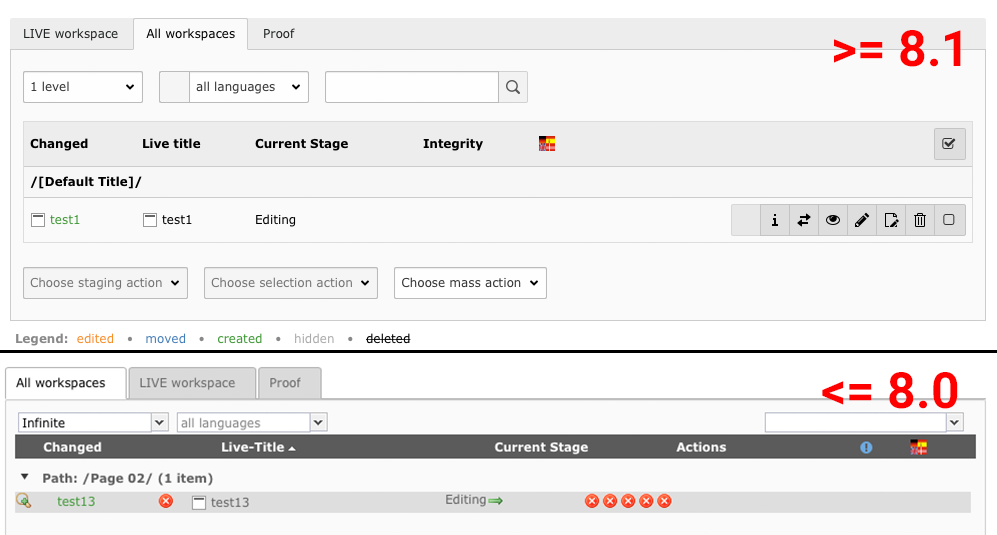
\includegraphics[width=0.85\linewidth]{BackendUserInterface/workspaces.png}
	\end{figure}

\end{frame}

% ------------------------------------------------------------------------------
